% !TEX program = pdflatex
% !TEX root = staged_reward_paper_en.tex

\documentclass{article}

% Allow compiling either from paper/ or from the repository root.
\makeatletter
\def\input@path{{./}{paper/}}
\makeatother

\usepackage[preprint,nonatbib]{neurips_2026}

\usepackage[utf8]{inputenc}
\usepackage[T1]{fontenc}
\usepackage{amsmath}
\usepackage{amssymb}
\usepackage{booktabs}
\usepackage{graphicx}
\usepackage{tabularx}
\usepackage{array}
\usepackage{makecell}
\usepackage{enumitem}
\usepackage{xcolor}
\usepackage{hyperref}
\usepackage{url}

\hypersetup{hidelinks}
\graphicspath{{./}}
\setlist[itemize]{leftmargin=1.5em}
\setlist[enumerate]{leftmargin=1.8em}
\newcommand{\relu}[1]{\left[#1\right]_+}
\newcommand{\ind}{\mathbf{1}}

\title{Stable Arm Swing Humanoid Locomotion under Upper Body Perturbations}

\author{%
  Yuhao Chao\thanks{Equal contribution.} \\
  Shanghai Innovation Institute \\
  Fudan University \\
  \texttt{CZXS25230326}
  \And
  Zhetao Chen\footnotemark[1] \\
  Shanghai Innovation Institute \\
  Zhejiang University \\
  \texttt{CZXS25230081}
}

\begin{document}

\maketitle

\begin{abstract}
Unlocking joints in the upper body changes humanoid locomotion from velocity tracking for the legs into a coordination problem for the whole body. Arm motion can alter torso attitude, angular momentum distribution, and foot contact timing; when arm swing objectives are simply added to a conventional locomotion reward, reinforcement learning policies often discover lateral drift, torso compensation, rapid arm motion, or overly rigid arms that avoid stability penalties. We introduce a three stage reward curriculum for the H1 humanoid in a full 19 DoF action space. The policy first learns stable forward walking while the upper body is constrained, then activates arm swing rewards only in compatible command contexts through gait conditioned reward routing, and finally learns to recover from random pulse perturbations applied to torso, shoulder, and elbow action channels. All stages are trained with PPO from reward signals alone, without motion capture trajectories, expert demonstrations, or imitation losses. In 32 parallel environments over a 20 s evaluation horizon, the final policy preserves a 100\% survival rate under perturbation amplitude 2.0, achieves a forward velocity tracking error of 0.0245 m/s, keeps maximum body tilt below 10 deg, and retains visible shoulder swing and sagittal motion of the arm endpoints. The result is a pure RL pipeline in which arm swing emerges from staged reward routing and robustness learning rather than from a single reward weight sweep.
\end{abstract}

\textbf{Keywords:} humanoid locomotion; reinforcement learning; reward design; arm swing; gait conditioned routing; upper body perturbation; robust walking

\section{Introduction}

Humanoid locomotion policies usually prioritize velocity tracking, body attitude stability, and reliable ground contact. Once the task expands from legged walking to coordinated motion of the whole body, however, the degrees of freedom in the upper body make the control problem substantially harder. In the H1 robot used in this work, the lower body baseline controls only 10 leg joints, whereas the full model exposes 19 controllable joints, including the torso, bilateral shoulder pitch/roll/yaw joints, and bilateral elbows. Directly unlocking these joints does not automatically produce humanlike arm swing. A reinforcement learning policy optimizes cumulative reward, so it can keep the arms rigid to avoid penalties, swing laterally, twist the torso, or exploit rapid motions that locally improve reward without producing stable coordination.

Deep reinforcement learning has become a practical tool for legged and bipedal locomotion when training is made efficient and robust in simulation~\cite{rudin2022learning,li2021reinforcement}. In contrast, many approaches that aim for natural whole-body motion rely on example trajectories, motion priors, or animal and human demonstrations~\cite{peng2018deepmimic,peng2020learningagile,peng2021amp}. This paper takes the complementary route: we ask whether visible arm swing and upper-body recovery can be obtained by pure reinforcement learning from staged rewards, without demonstration data.

Our central hypothesis is that arm swing is not an isolated action. It is a gait conditioned behavior of the whole body, coupled to the current command, contact rhythm, and stability constraints. For that reason, arm swing rewards should not be active in every state. They should be routed into the contexts in which arm swing is useful, after a stable locomotion substrate has already been learned. Building on this hypothesis, we design a curriculum that moves from stable walking with the lower body, to arm swing conditioned on commands, to recovery from perturbations in the upper body.

We make four contributions:
\begin{enumerate}
  \item We train in the full 19 DoF H1 action space from the beginning, avoiding the action space and dynamics mismatch caused by directly transferring a 10 DoF policy for the lower body.
  \item We adapt gait conditioned reward routing~\cite{peng2025gait} to arm swing in the upper body by constructing command based masks for standing, walking, and straight walking contexts.
  \item We design a pure reinforcement learning solution without reference motions or demonstration data, approximating visible arm swing through shoulder phase coupling, left and right velocity opposition, and sagittal displacement of elbow endpoints.
  \item We introduce random pulse perturbations at the action level of the upper body and evaluate survival, velocity tracking, and posture stability under torso, shoulder, and elbow disturbances.
\end{enumerate}

\begin{figure}[t]
  \centering
  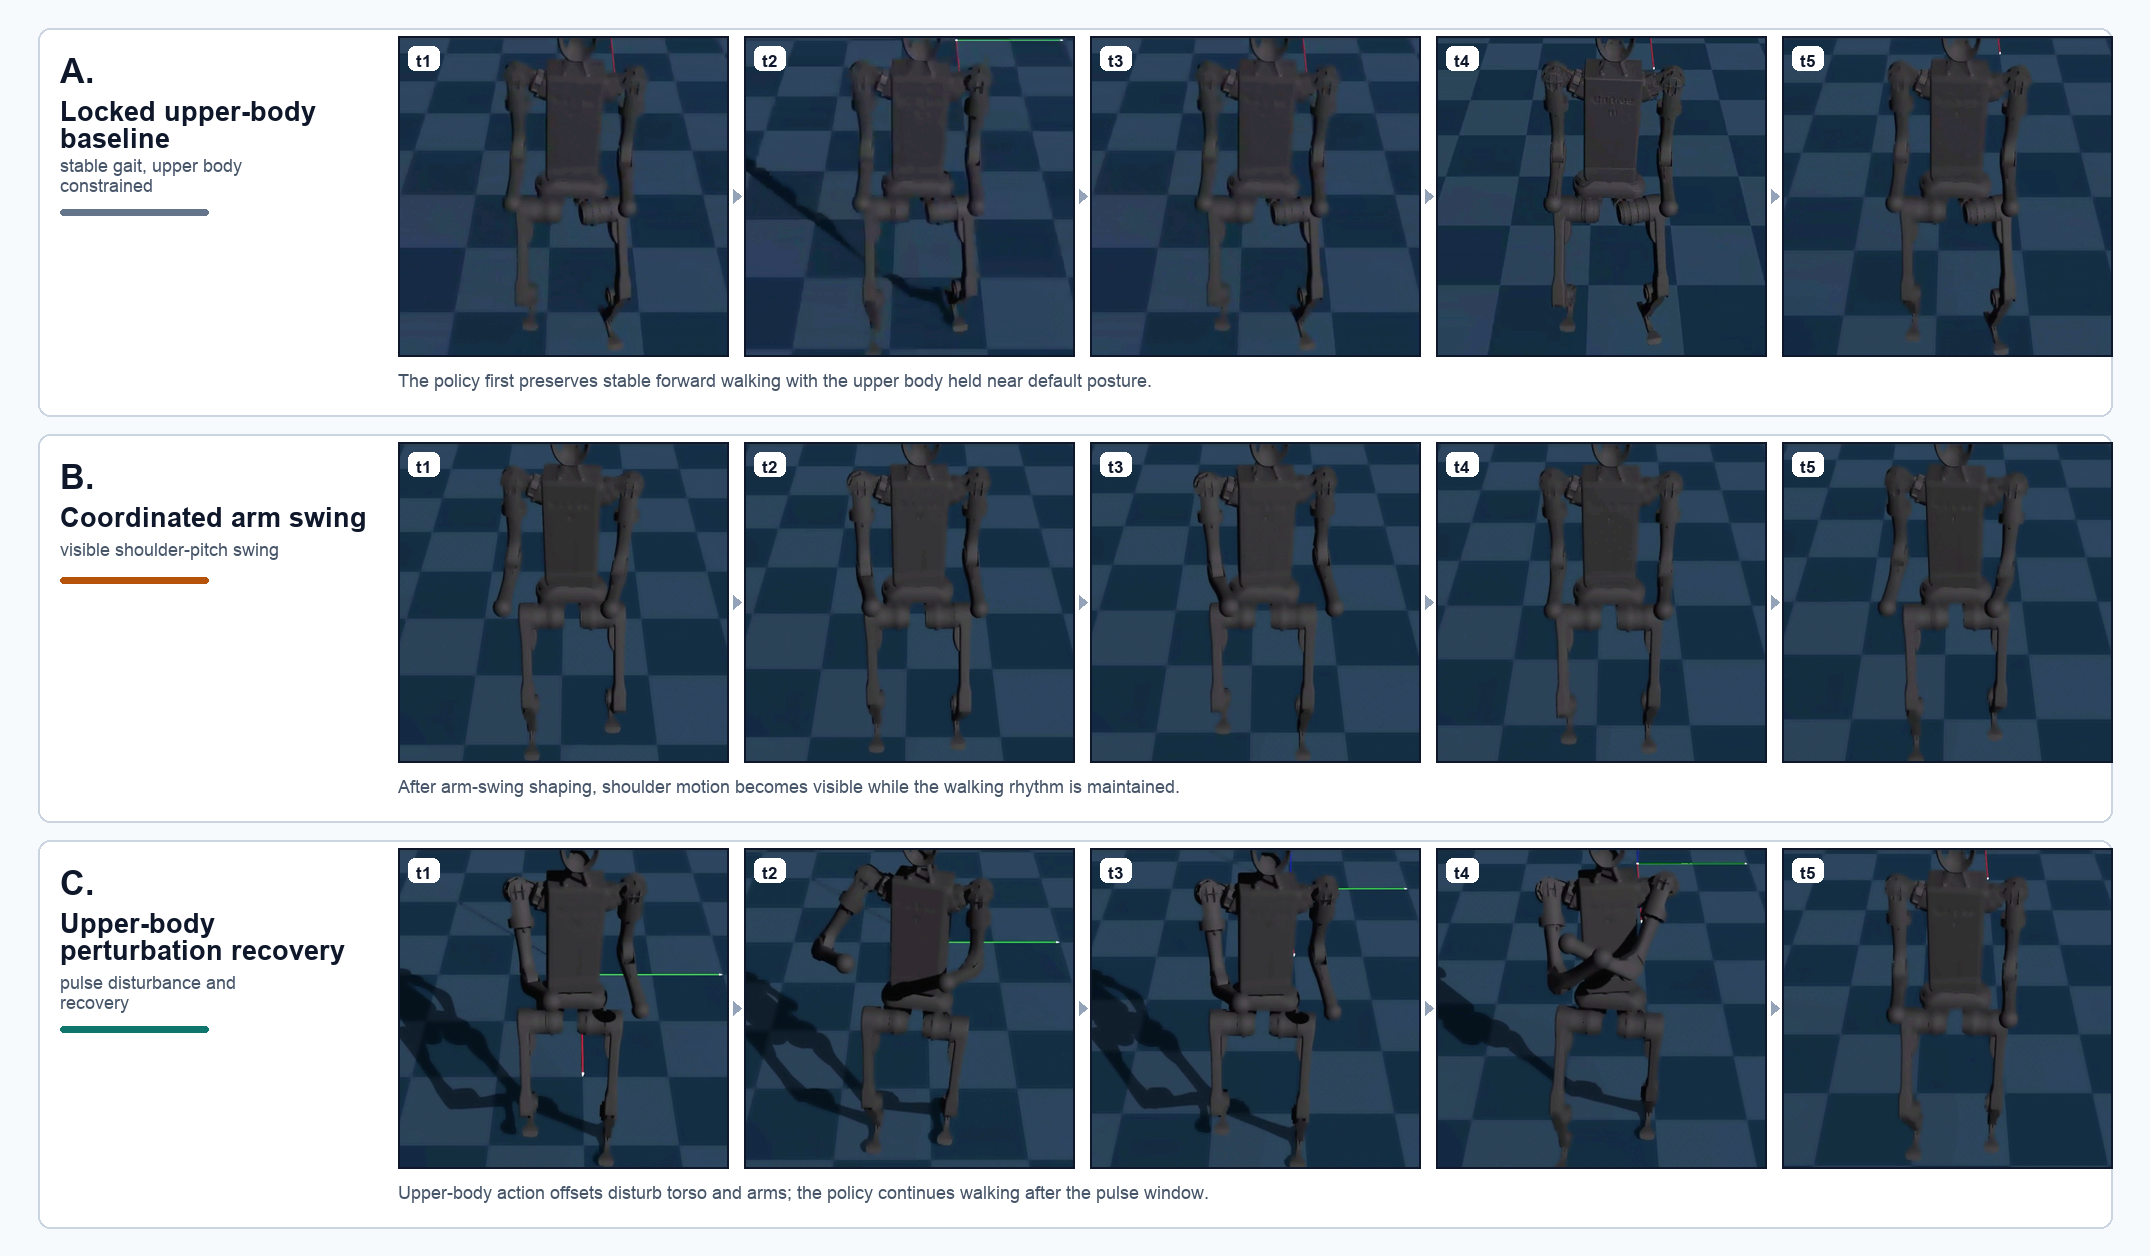
\includegraphics[width=\linewidth]{figure1_temporal_montage.png}
  \caption{Behavioral evidence across the three stage curriculum. The first row shows stable walking with the upper body constrained. The second row shows visible shoulder swing during straight walking. The third row shows continued forward motion and recovery after pulse perturbations in the upper body.}
  \label{fig:temporal}
\end{figure}

\section{Problem Formulation}

We formulate locomotion control for the whole body as a partially observable Markov decision process:
\begin{equation}
\mathcal{M}=(\mathcal{S},\mathcal{A},P,r,\gamma,p_0),
\end{equation}
where $s_t\in\mathcal{S}$ is the robot state, $a_t\in\mathcal{A}$ is the joint action produced by the policy, $P$ denotes the transition dynamics, $r_t$ is the instantaneous reward, and $\gamma$ is the discount factor. The policy $\pi_\theta(a_t\mid o_t)$ maps proprioceptive observations $o_t$ to 19 DoF joint actions and maximizes
\begin{equation}
J(\theta)=
\mathbb{E}_{\pi_\theta}
\left[
\sum_{t=0}^{T-1}\gamma^t r_t
\right].
\end{equation}

The action space decomposes into leg and upper body subsets:
\begin{equation}
\mathcal{A}=\mathcal{A}_{\mathcal{L}}\times\mathcal{A}_{\mathcal{U}},
\qquad
\mathcal{U}=\{\text{torso},\text{shoulder},\text{elbow}\}.
\end{equation}
The objective is not to maximize a single arm swing metric. Instead, the policy must preserve locomotion stability while making upper body motion satisfy gait coordination and recovery constraints after disturbances. No demonstration trajectories are provided; the desired coordination emerges only from reinforcement learning on the staged reward. We therefore design the reward as a staged composition of increasingly demanding objectives.

\section{Staged Reward Design}

\subsection{Reward Decomposition}

We use the following unified reward form:
\begin{equation}
\begin{aligned}
r_t ={}&
r_{\mathrm{track},t}
+ r_{\mathrm{safe},t}
+ m_{\mathrm{stand},t} r_{\mathrm{stand},t}
+ m_{\mathrm{walk},t} r_{\mathrm{walk},t} \\
&+ m_{\mathrm{straight},t} r_{\mathrm{swing},t}
+ r_{\mathrm{robust},t} .
\end{aligned}
\label{eq:reward-decompose}
\end{equation}
Here $r_{\mathrm{track},t}$ measures velocity and heading tracking, while $r_{\mathrm{safe},t}$ captures posture, joint limits, action smoothness, and upper body safety constraints. The terms $r_{\mathrm{stand},t}$, $r_{\mathrm{walk},t}$, and $r_{\mathrm{swing},t}$ correspond to standing, walking, and arm swing during straight walking. The term $r_{\mathrm{robust},t}$ strengthens stable recovery during the perturbation stage. The masks $m_{\mathrm{stand},t}$, $m_{\mathrm{walk},t}$, and $m_{\mathrm{straight},t}$ ensure that each behavior specific reward is optimized only in its matching command context.

\begin{figure}[t]
  \centering
  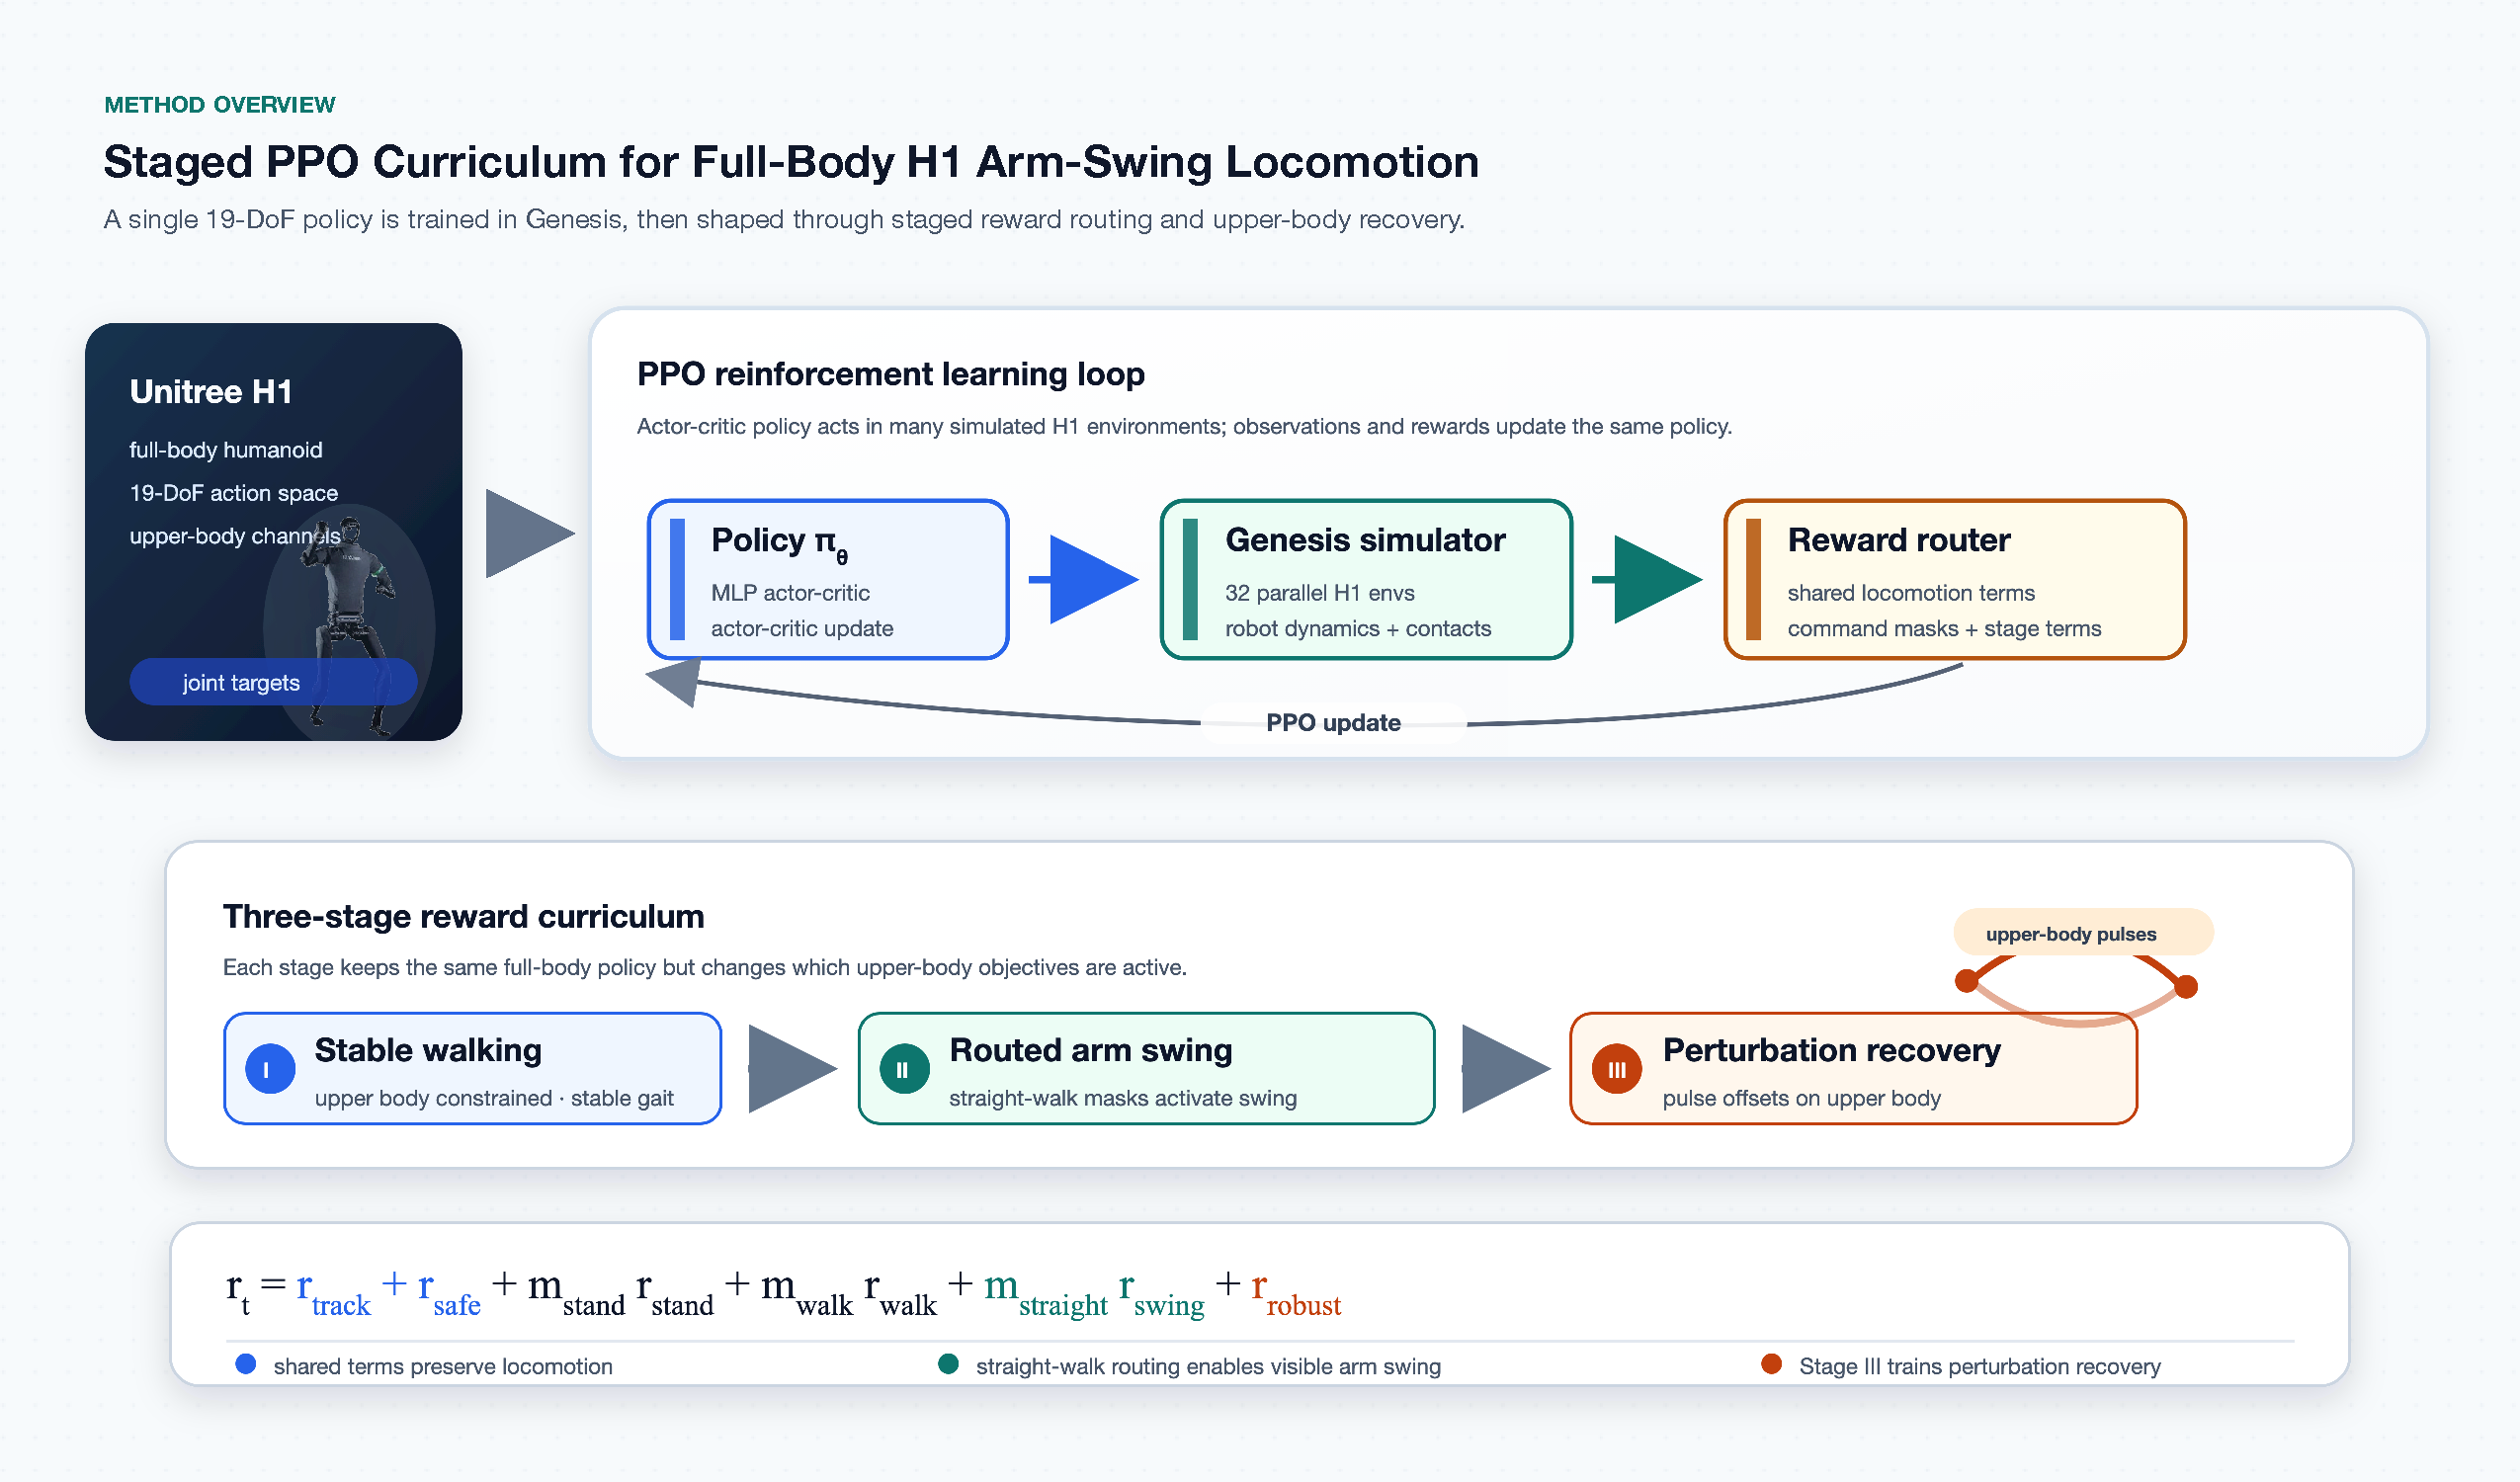
\includegraphics[width=\linewidth]{method_overview.pdf}
  \caption{Method overview. PPO trains a single 19 DoF Unitree H1 policy in Genesis from reward feedback alone, without demonstration data. The staged curriculum first establishes stable walking, then routes arm swing rewards to straight walking commands, and finally adds pulse perturbations on upper body action channels to train and evaluate recovery.}
  \label{fig:routing}
\end{figure}

\subsection{Stage I: Stable Lower Body Walking}

The first stage establishes stable forward walking in the full 19 DoF model. Although the action space already contains joints in the upper body, the torso, shoulders, and elbows are constrained near their default poses during this stage. The reward can be summarized as
\begin{equation}
r_t^{(1)} =
r_{\mathrm{track},t}
+ r_{\mathrm{base},t}
+ r_{\mathrm{foot},t}
- c_{\mathrm{upper-lock},t}
- c_{\mathrm{smooth},t} .
\end{equation}
The velocity and heading tracking term is written as
\begin{equation}
r_{\mathrm{track},t}
=
w_x \exp\left(-\frac{|v_{x,t}-v_{x,t}^{\mathrm{cmd}}|}{\sigma_x}\right)
+ w_\psi \exp\left(-\frac{|\psi_t-\psi_t^{\mathrm{cmd}}|}{\sigma_\psi}\right),
\end{equation}
and the upper body locking cost is
\begin{equation}
c_{\mathrm{upper-lock},t}
=
\sum_{j\in\mathcal{U}}
\relu{|q_{j,t}-q_j^0|-\epsilon_j}^2 .
\end{equation}
Here $q_j^0$ is the default joint angle and $\relu{\cdot}=\max(\cdot,0)$. This design allows the policy to learn locomotion in the full robot model while preventing early exploration from using the upper body as an unstable compensator.

\subsection{Stage II: Arm Swing Conditioned on Commands}

The second stage releases the left and right shoulder pitch joints while keeping the torso, shoulder roll/yaw, and elbows constrained. The key design choice is not to increase a global arm swing weight, but to route the arm swing reward into straight walking contexts. We define masks conditioned on commands as
\begin{align}
m_{\mathrm{stand},t}
&=
\ind\left[\left\|\mathbf{v}_{xy,t}^{\mathrm{cmd}}\right\|_2
\le v_{\mathrm{stand}}\right],\\
m_{\mathrm{walk},t}
&=
\ind\left[\left\|\mathbf{v}_{xy,t}^{\mathrm{cmd}}\right\|_2
> v_{\mathrm{walk}}\right],\\
m_{\mathrm{straight},t}
&=
\ind\left[
v_{x,t}^{\mathrm{cmd}}>v_{\min}
\land |v_{y,t}^{\mathrm{cmd}}|<\epsilon_y
\land |\omega_{z,t}^{\mathrm{cmd}}|<\epsilon_\omega
\right].
\end{align}

The arm swing reward contains three main error terms. First, shoulder motion is coupled to the contralateral hip phase:
\begin{equation}
e_{\mathrm{phase},t}
=
\left(q_{L,t}^{\mathrm{sh}}-k q_{R,t}^{\mathrm{hip}}\right)^2
+
\left(q_{R,t}^{\mathrm{sh}}-k q_{L,t}^{\mathrm{hip}}\right)^2 .
\end{equation}
Second, the left and right shoulder pitch velocities are encouraged to be approximately out of phase:
\begin{equation}
e_{\mathrm{opp},t}
=
\left(\dot q_{L,t}^{\mathrm{sh}}+\dot q_{R,t}^{\mathrm{sh}}\right)^2 .
\end{equation}
Third, the sagittal displacement between the left and right elbow endpoints in the robot base frame should exceed a minimum visible swing amplitude:
\begin{equation}
e_{\mathrm{amp},t}
=
\relu{
\delta_{\min}
-
\left|x_{L,t}^{\mathrm{elbow}}-x_{R,t}^{\mathrm{elbow}}\right|
}^2 .
\end{equation}
The resulting arm swing term is
\begin{equation}
r_{\mathrm{swing},t}
=
-w_{\mathrm{phase}}e_{\mathrm{phase},t}
-w_{\mathrm{opp}}e_{\mathrm{opp},t}
-w_{\mathrm{amp}}e_{\mathrm{amp},t},
\end{equation}
and it is activated only under $m_{\mathrm{straight},t}$. This design follows the reward routing intuition of gait conditioned reinforcement learning: different command regimes imply different behavioral objectives, so reward terms should switch with context rather than remain globally active.

\subsection{Stage III: Upper Body Perturbation Recovery}

The third stage inherits the arm swing objective from Stage II and injects random pulse perturbations into action channels in the upper body. Given a policy action $a_t$, the executed action $\tilde a_t$ is
\begin{equation}
\tilde a_{t,j}=
\begin{cases}
\mathrm{clip}(a_{t,j}+s_j\eta_{t,j},-a_{\max},a_{\max}), & j\in\mathcal{U},\\
a_{t,j}, & j\in\mathcal{L},
\end{cases}
\end{equation}
where $\eta_{t,j}\sim\mathcal{U}(-\alpha,\alpha)$ is a random action offset, $s_j$ is a perturbation scale for each joint, and $\alpha$ controls perturbation amplitude. The perturbation is applied as a pulse: a random offset is held for a short active window, then disabled to provide a recovery window. This pulse structure separates the disturbed phase from the recovery phase more explicitly than continuous noise.

Stage III strengthens terms for straight walking and posture stability:
\begin{equation}
r_{\mathrm{robust},t}
=
w_v r_{v_x,t}
+ w_h r_{\mathrm{heading},t}
-\lambda_o c_{\mathrm{orientation},t}
-\lambda_y |v_{y,t}|
-\lambda_s \relu{v_{\min}-v_{x,t}} .
\end{equation}
The goal is not to maximize arm amplitude. Instead, the policy must maintain forward velocity, limit lateral drift, and keep body tilt controlled after random action offsets in the upper body.

\section{Relation to Gait Conditioned Reward Routing}

Gait conditioned reward routing addresses reward interference in locomotion with multiple gaits or behaviors. Standing favors stillness and stable double support, walking favors periodic foot motion and forward velocity, and running favors shorter contact and stronger push off. If all reward terms tied to a gait remain active at once, the policy receives conflicting optimization signals. The gait conditioned approach uses gait identifiers and reward masks so that a shared policy optimizes different objectives under different gait modes~\cite{peng2025gait}.

Our method does not reproduce the full gait identifier, recurrent policy, or centroidal angular momentum reward used in that setting. Instead, we translate the same idea into a lighter routing scheme based on commands. The task contains a smaller set of contexts: standing, straight walking, arm swing, and perturbation recovery. These contexts can be inferred directly from velocity commands, so we avoid changing the observation space. The resulting routing keeps arm swing rewards from being forced during standing or complex turns, while preventing standing stability rewards from suppressing necessary coordination in the upper body during walking.

\section{Experimental Setup}

We train an H1 policy for the whole body in the Genesis simulator using PPO~\cite{schulman2017proximal}. The training pipeline does not load expert trajectories, motion capture clips, or offline demonstration datasets. The policy controls 19 joints and is evaluated in 32 parallel environments. Each evaluation lasts 1000 steps, corresponding to a 20 s horizon. The commanded velocity is fixed to $[0.6,0,0]$ m/s. Perturbations are applied only to torso, shoulder, and elbow action channels; actions for the lower body are not directly perturbed. We report three categories of metrics.

The survival rate is
\begin{equation}
S=\frac{1}{N}\sum_{i=1}^{N}\ind[T_i\ge T],
\end{equation}
where $T_i$ denotes the first reset time of environment $i$ that is not due to timeout. The forward velocity tracking error is
\begin{equation}
E_{v_x}=
\frac{1}{NT}
\sum_{i=1}^{N}\sum_{t=1}^{T}
\left|v_{x,t}^{(i)}-v_x^{\mathrm{cmd}}\right|.
\end{equation}
Body tilt is approximated from the horizontal components of projected gravity:
\begin{equation}
\theta_t=
\arcsin\left(
\left\|\mathbf{g}_{xy,t}^{\mathrm{proj}}\right\|_2
\right).
\end{equation}
The recovery success rate measures whether the robot regains velocity and attitude thresholds after each perturbation pulse:
\begin{equation}
\rho=
\frac{1}{K}
\sum_{k=1}^{K}
\ind
\left[
v_{x,t_k}^{\mathrm{rec}}\ge 0.8 v_x^{\mathrm{cmd}}
\land
\theta_{t_k}^{\mathrm{rec}}\le \theta_{\max}
\right].
\end{equation}

\section{Results}

\begin{figure}[t]
  \centering
  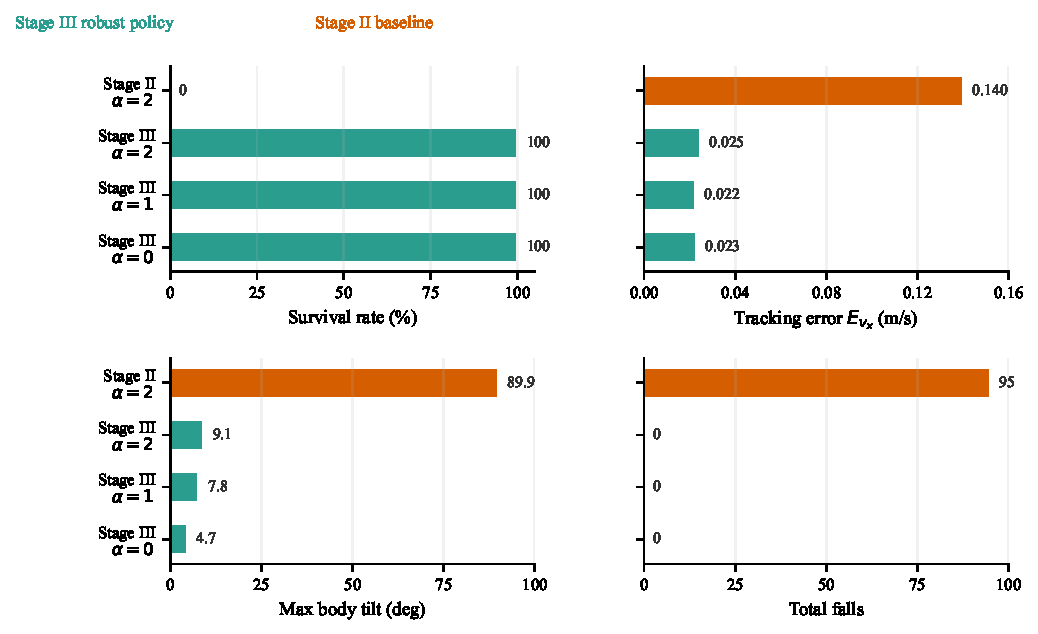
\includegraphics[width=\linewidth]{quantitative_results.pdf}
  \caption{Bar chart summary of finite horizon perturbation evaluation. Each row label combines policy and perturbation amplitude; the horizontal axis reports the value of the corresponding metric. The detailed numerical values are reported separately in Table~\ref{tab:robust}.}
  \label{fig:quant}
\end{figure}

\begin{table}[t]
  \caption{Finite horizon evaluation and upper body motion metrics.}
  \label{tab:robust}
  \centering
  \scriptsize
  \textit{(a) Perturbation robustness.}\\[2pt]
  \resizebox{\linewidth}{!}{%
  \begin{tabular}{lccccccc}
    \toprule
    Policy & Perturb. amp. $\alpha$ & Survival $\uparrow$ & Mean survival $\uparrow$ & $E_{v_x}$ $\downarrow$ & Mean lateral vel. $\downarrow$ & Max tilt $\downarrow$ & Total falls $\downarrow$ \\
    \midrule
    Stage III & 0.0 & 100.0\% & 20.00 s & 0.0228 m/s & 0.0508 m/s & 4.67 deg & 0 \\
    Stage III & 1.0 & 100.0\% & 20.00 s & 0.0225 m/s & 0.0542 m/s & 7.81 deg & 0 \\
    Stage III & 2.0 & 100.0\% & 20.00 s & 0.0245 m/s & 0.0564 m/s & 9.12 deg & 0 \\
    Stage II baseline & 2.0 & 0.0\% & 5.48 s & 0.1401 m/s & 0.1335 m/s & 89.93 deg & 95 \\
    \bottomrule
  \end{tabular}}
  \vspace{4pt}

  \textit{(b) Arm swing metrics.}\\[2pt]
  \resizebox{\linewidth}{!}{%
  \begin{tabular}{lccccc}
    \toprule
    Policy & Perturb. amp. $\alpha$ & Mean upper action offset & Shoulder swing amp. & Arm opposition error $\downarrow$ & Elbow sagittal span \\
    \midrule
    Stage III & 0.0 & 0.0000 & 0.2317 rad & 0.4239 rad & 0.1035 m \\
    Stage III & 1.0 & 0.1095 & 0.2141 rad & 0.3249 rad & 0.1098 m \\
    Stage III & 2.0 & 0.2168 & 0.2536 rad & 0.3952 rad & 0.1165 m \\
    Stage II baseline & 2.0 & 0.2079 & 0.2638 rad & 0.2997 rad & 0.1459 m \\
    \bottomrule
  \end{tabular}}
\end{table}

Table~\ref{tab:robust} shows that Stage III preserves a 100\% survival rate at perturbation amplitude $\alpha=2.0$. The forward velocity tracking error increases only from 0.0228 m/s without perturbation to 0.0245 m/s under the strongest tested perturbation, and the maximum body tilt remains 9.12 deg. In contrast, the Stage II baseline already exhibits visible arm swing but fails in every environment under the same perturbation amplitude; its mean survival time drops to 5.48 s and it accumulates 95 falls. Panel (b) shows that the robustness of Stage III is not achieved by eliminating motion in the upper body. At $\alpha=2.0$, the policy still maintains a 0.2536 rad shoulder swing amplitude and a 0.1165 m sagittal span between elbow endpoints.

\section{Analysis of Failed Designs}

Before arriving at the final three stage curriculum, we evaluated several exploratory reward variants. These variants did not reliably produce natural arm swing because their reward terms lacked context routing or because arm swing objectives conflicted with stability constraints.

\begin{table}[t]
  \caption{Main failure modes of exploratory reward trials.}
  \label{tab:failed}
  \centering
  \small
  \begin{tabularx}{\linewidth}{lXX}
    \toprule
    Trial & Design intent & Main issue \\
    \midrule
    Trial 2 & Release only shoulder pitch and add weak phase and endpoint constraints & The arm swing signal is weak and is easily suppressed by smoothness, limit, and centering penalties \\
    Trial 3 & Release more arm joints and strengthen endpoint and lateral constraints & Rewards for the upper body become numerous and mixed in direction, so the policy tends toward stiffness or local penalty avoidance \\
    Trial 4 & Use a fixed sinusoidal teacher to shape shoulder pitch & The teacher is not synchronized with contact phase or velocity command, which can disrupt gait naturalness \\
    Trial 5 & Reduce the teacher amplitude for more conservative arm motion & The arm swing signal becomes weaker while global reward interference remains unresolved \\
    \bottomrule
  \end{tabularx}
\end{table}

These failures indicate that arm swing learning cannot be reduced to increasing a single reward weight. When standing, walking, turning, and perturbation recovery share one global reward mixture, the policy receives contradictory gradients. A more effective design first protects locomotion, then activates arm and leg coordination only during straight walking, and finally trains disturbance recovery as a separate robustness objective.

\section{Discussion}

A useful property of the proposed method is interpretability. Each stage corresponds to a clear behavioral hypothesis: Stage I verifies that the full model can preserve stable locomotion in the lower body; Stage II tests whether reward routing conditioned on commands can produce visible arm swing; and Stage III tests whether the resulting arm swing policy can recover from action pulses in the upper body. Compared with motion capture imitation or adversarial motion priors~\cite{peng2021amp}, our method is pure reinforcement learning: it does not require external motion data, demonstrations, or a discriminator trained on reference clips. This choice lowers implementation cost and makes the connection between reward terms and failure modes easier to inspect. Hierarchical or compositional policy methods~\cite{peng2019mcp} provide another route for skill organization, but our design keeps a single compact PPO policy and uses routing only at the reward level.

The method still has clear limitations. First, it remains a hand designed reward shaping approach. The naturalness of arm swing is approximated through shoulder pitch phase, velocity opposition, and endpoint displacement; the policy does not explicitly optimize centroidal angular momentum of the whole body. Second, all experiments are restricted to simulation and use a short finite horizon, so the results should not be interpreted as evidence of transfer to a real robot. Third, the current routing scheme depends on velocity command thresholds. More complex turning, variable speed, or uneven terrain tasks may require richer gait state representations.

\section{Conclusion}

We presented a three stage reward curriculum for H1 humanoid locomotion that moves from stable walking with the lower body to visible arm swing and finally to robustness against random action perturbations in the upper body. The central conclusion is that arm swing should be treated as a gait conditioned coordination behavior of the whole body, not as an isolated joint trajectory tracking objective. By first constraining the upper body to establish a stable locomotion substrate, then activating arm swing rewards through routing based on commands, and finally training recovery under pulse perturbations, the final policy maintains full survival and low velocity tracking error under strong perturbations to the upper body while preserving visible arm swing. Together, the results make staged rewards, command routing, and explicit pulse recovery a compact pure RL recipe for coordinated humanoid locomotion without demonstration data.

\IfFileExists{staged_reward_paper.bib}{%
  \bibliographystyle{plain}
  \bibliography{staged_reward_paper}
}{%
  \bibliographystyle{plain}
  \bibliography{paper/staged_reward_paper}
}

\end{document}
